\documentclass[xcolor=table]{beamer}

\usepackage{booktabs}
\usepackage{hyperref}
\usepackage[table]{xcolor}
\usepackage{tikz}
\usepackage{graphics}
\usetikzlibrary{calc}

\setbeamertemplate{navigation symbols}{}%remove navigation symbols

\title{Extensive Form Games}
\subtitle{Game Theory}
\author{Vincent Knight}
\date{}

\tikzstyle{level 1}=[level distance=3.5cm, sibling distance=3.5cm]
\tikzstyle{level 2}=[level distance=3.5cm, sibling distance=2cm]
\tikzstyle{player} = [text width=4em, draw, text centered, rectangle, fill=blue!20, inner sep=1pt]
\tikzstyle{nature} = [minimum width=3pt,circle,  draw, fill=red!20, inner sep=1pt]
\tikzstyle{end} = [circle, minimum width=3pt, fill, inner sep=0pt, right]
\tikzstyle{dot} = [draw,shape=circle,fill=blue]

\begin{document}

\frame{\titlepage}

\frame{
\begin{center}
\tikzstyle{level 1}=[level distance=3.5cm, sibling distance=3.5cm]
\tikzstyle{level 2}=[level distance=3.5cm, sibling distance=2cm]
\tikzstyle{player} = [text width=5em, draw, text centered, rectangle, fill=blue!20, inner sep=1pt]
\tikzstyle{nature} = [minimum width=3pt,circle,  draw, fill=red!20, inner sep=1pt]
\tikzstyle{end} = [circle, minimum width=3pt, fill, inner sep=0pt, right]
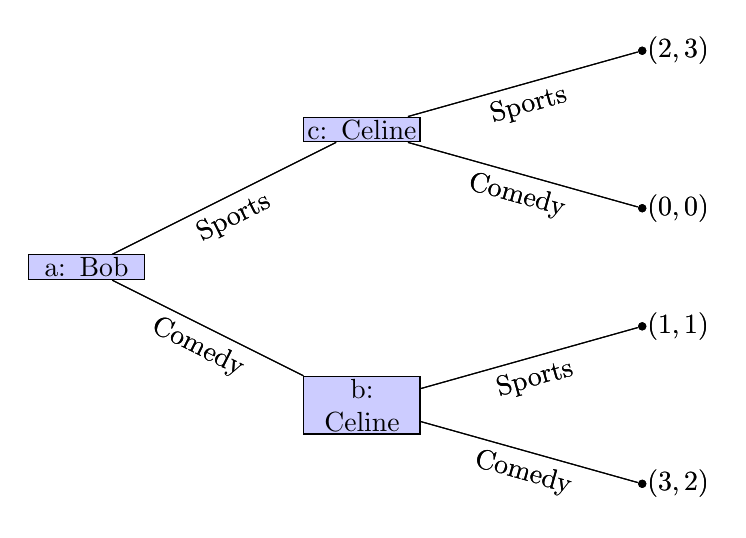
\begin{tikzpicture}[grow=right, sloped]
    \node[player]{a: Bob}
        child {node[player] {b: Celine}
                child {node[end] {} node[right] {$(3,2)$} edge from parent node[below] {Comedy}}
                child {node[end] {} node[right] {$(1,1)$} edge from parent node[below] {Sports}} edge from parent node[below] {Comedy}}
        child {node[player] {c: Celine}
                child {node[end] {} node[right] {$(0,0)$} edge from parent node[below] {Comedy}}
                child {node[end] {} node[right] {$(2,3)$} edge from parent node[below] {Sports}} edge from parent node[below] {Sports}};
    \node[player]{a: Bob}
        child {node[player] {b: Celine}
                child {node[end] {} node[right] {$(3,2)$} edge from parent node[below] {Comedy}}
                child {node[end] {} node[right] {$(1,1)$} edge from parent node[below] {Sports}} edge from parent node[below] {Comedy}}
        child {node[player] {c: Celine}
                child {node[end] {} node[right] {$(0,0)$} edge from parent node[below] {Comedy}}
                child {node[end] {} node[right] {$(2,3)$} edge from parent node[below] {Sports}} edge from parent node[below] {Sports}};
\end{tikzpicture}
\end{center}
}

\frame{

\begin{itemize}
\item \textbf{Sequential rationality:} An optimal strategy for a player should maximise that player's expected payoff, conditional on every information set at which that player has a decision.

\item \textbf{Backward induction:} This is the process of analysing a game from back to front. At each information set we remove strategies that are dominated.
\end{itemize}
}

\begin{frame}
\tikzstyle{level 1}=[level distance=2cm, sibling distance=3.5cm]
\tikzstyle{level 2}=[level distance=2cm, sibling distance=2cm]
\tikzstyle{player} = [text width=5em, draw, text centered, rectangle, fill=blue!20, inner sep=1pt]
\tikzstyle{nature} = [minimum width=3pt,circle,  draw, fill=red!20, inner sep=1pt]
\tikzstyle{end} = [circle, minimum width=3pt, fill, inner sep=0pt, right]
\tikzstyle{corner} = [inner sep=0pt, outer sep=0pt, draw,circle]
\begin{center}
\begin{tikzpicture}[grow=right, sloped]
    \node[player]{Leader}
                child {node [corner] (A1) {}  }
                child {node [corner] (A2) {} edge from parent node[above] {$a$}} ;
        \draw [bend right] (A1) to (A2);
        \node (B3) [player,right=3pt] at ($(A1)!0.5!(A2)$) {Follower}
            child {node [corner] (A3) {}  }
            child {node [corner] (A4) {} edge from parent node[above] {$b$}} ;
        \draw [bend right] (A3) to (A4);
        \node (e) [end,right=13pt] at ($(A3)!0.5!(A4)$) {} ;
        \node [right] at (e) {$(2ab-8b^2+3a,ab-b^2)$};
\end{tikzpicture}
\end{center}
\pause
$$\frac{d}{db}(ab-b^2)=0\Rightarrow b^*=\frac{a}{2}$$
\end{frame}

\begin{frame}
\tikzstyle{level 1}=[level distance=2cm, sibling distance=3.5cm]
\tikzstyle{level 2}=[level distance=2cm, sibling distance=2cm]
\tikzstyle{player} = [text width=5em, draw, text centered, rectangle, fill=blue!20, inner sep=1pt]
\tikzstyle{nature} = [minimum width=3pt,circle,  draw, fill=red!20, inner sep=1pt]
\tikzstyle{end} = [circle, minimum width=3pt, fill, inner sep=0pt, right]
\tikzstyle{corner} = [inner sep=0pt, outer sep=0pt, draw,circle]
\begin{center}
\begin{tikzpicture}[grow=right, sloped]
    \node[player]{Leader}
                child {node [corner] (A1) {}  }
                child {node [corner] (A2) {} edge from parent node[above] {$a$}} ;
        \draw [bend right] (A1) to (A2);
        \node (e) [end,right=13pt] at ($(A1)!0.5!(A2)$) {} ;
        \only<1-2>{\node [right] at (e) {$(2ab-8b^2+3a,ab-b^2)$};}
        \onslide<2>{
        \node (A) at (5,2) {$b^*=a/2$};
        \draw (A) edge[out=135,in=90,->,color=red] (3.2,.2);
        \draw (A) edge[out=-45,in=90,->,color=red] (4.2,.2);
        \draw (A) edge[out=-45,in=90,->,color=red] (6.4,.2);
        \draw (A) edge[out=-45,in=90,->,color=red] (5.7,.2);
        }
        \only<3->{\node [right] at (e) {$(a^2-2a^2+3a,a^2/2-a^2/4)$};}
\end{tikzpicture}
\end{center}
\onslide<3->{
$$\frac{d}{da}(-a^2+3a)=0\Rightarrow a^*=\frac{2}{3}$$
}
\onslide<4->{
\begin{center}
\framebox{$(a^*,b^*)=(2/3,2/6)$}
\end{center}
}
\end{frame}

\end{document}
